\documentclass[12pt, letterpaper]{../assignment}
\usepackage{graphicx}
\usepackage{courier}
\usepackage{minted}
\usepackage{amsmath}
\usepackage{polynom}
\usepackage{commath}
\usepackage{amssymb}
\usepackage{amsfonts} 
\usepackage{color}
\usepackage{cancel}
\usepackage{enumitem}
\usepackage{graphicx}
\usepackage{multirow}
\usepackage{float}
\usepackage{bm}
\usepackage{tikz}
\usetikzlibrary{shapes,arrows}
\usepackage{booktabs}
\usetikzlibrary{patterns}

% Define Theme Colors
\definecolor{light-gray}{rgb}{0.2,0.2,0.2}
\definecolor{header-blue}{rgb}{0,0,0.7}
% \definecolor{header-blue}{rgb}{0.5137,0.8353,0.9176}
\definecolor{header-blue}{rgb}{0,0.8,0.95}
\definecolor{dark-gray}{rgb}{0.1,0.1,0.1}
\pagecolor{dark-gray}
\color{white}

\usemintedstyle{monokai}
\oddsidemargin = 0pt
\exercisesheet{Module 4}{Assignment}
\student{Austin Barrilleaux}
\university{\color{header-blue}Johns Hopkins University}
\school{\color{header-blue}Whiting School of Engineering}
\courselabel{EN 535.612}
\semester{Fall 2024}
\usepackage[backend=bibtex,style=numeric,sorting=none]{biblatex}
\bibliography{reference}

\definecolor{light-gray}{rgb}{0.2,0.2,0.2}
\setminted{bgcolor=light-gray,frame=lines,rulecolor=white}
\setlength{\parindent}{0pt}

\makeatletter
\patchcmd{\minted@colorbg}{\noindent}{\medskip\noindent}{}{}
\apptocmd{\endminted@colorbg}{\par\medskip}{}{}
\makeatother

\begin{document}

\subsection*{EXERCISE 4.39}
\subsubsection*{Gear A spins relative to its shaft,
which rotates at variable rate $\bm{\Omega_1}$ about the horizontal axis.
Gear B rotates at the variable rate $\bm{\Omega_2}$.
Determine the angular velocity and angular acceleration of gear A.}

\begin{figure}[H]
    \centering
    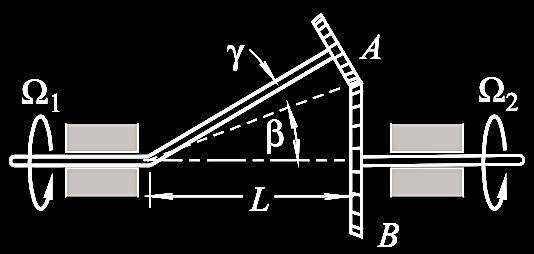
\includegraphics[frame]{images/Q4_39.png}
\end{figure}


\subsection*{EXERCISE 4.44}
\subsubsection*{The disk rolls without slipping over the horizontal XY plane.
At the instant when $\bm{\beta = 36.87^\circ}$,
the X and Y components of the velocity of point B on the horizontal diameter of the disk are 8 m/s and -4 m/s,
respectively, and the corresponding velocity components of center A at this instant are 4 m/s and 2 m/s.
Determine the precession angle $\bm{\Psi}$ between the horizontal diameter BAC and the X axis,
and also evaluate the precession, nutation, and spin rates.}

\begin{figure}[H]
    \centering
    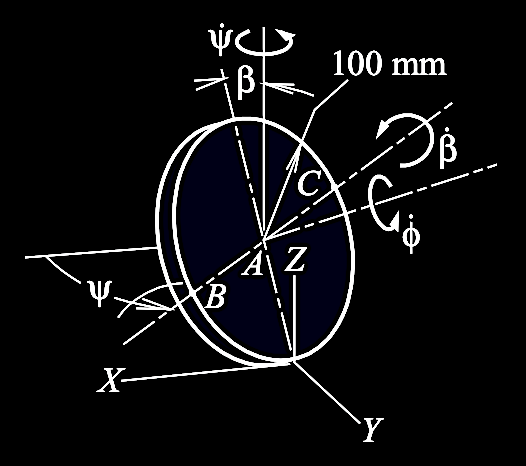
\includegraphics[scale=0.8,frame]{images/Q4_44.png}
\end{figure}

In the following sketch, we will define two coordinate frames, $\{XYZ\}$ and $\{xyz\}$:

\begin{center}

    \tikzset{every picture/.style={line width=0.75pt}} %set default line width to 0.75pt        

    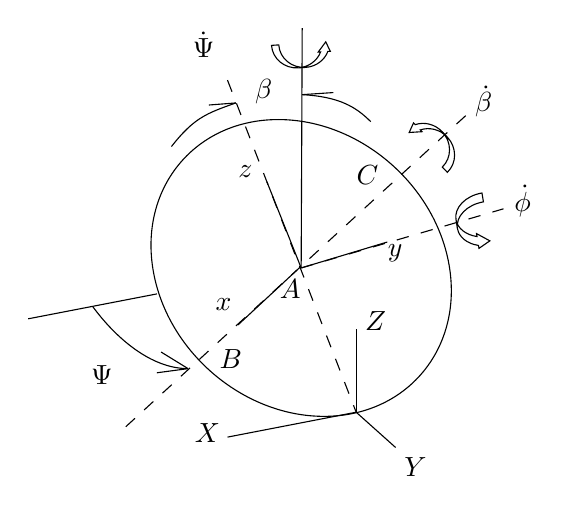
\begin{tikzpicture}[x=0.75pt,y=0.75pt,yscale=-1,xscale=1]
    %uncomment if require: \path (0,235); %set diagram left start at 0, and has height of 235
    
    %Shape: Circle [id:dp9205401865082012] 
    \draw   (163,119.5) .. controls (156.92,80.01) and (184.01,48) .. (223.5,48) .. controls (262.99,48) and (299.92,80.01) .. (306,119.5) .. controls (312.08,158.99) and (284.99,191) .. (245.5,191) .. controls (206.01,191) and (169.08,158.99) .. (163,119.5) -- cycle ;
    %Straight Lines [id:da08559310125076691] 
    \draw  [dash pattern={on 4.5pt off 4.5pt}]  (199,29) -- (261,189) ;
    %Straight Lines [id:da7745554258225504] 
    \draw    (234.5,119.5) -- (235,4) ;
    %Straight Lines [id:da5729101269761203] 
    \draw    (234.5,119.5) -- (218,78) ;
    %Straight Lines [id:da5020321684594107] 
    \draw    (199,201) -- (261,189) ;
    %Straight Lines [id:da6204394260932975] 
    \draw    (103,144) -- (165,132) ;
    %Straight Lines [id:da9164486645364178] 
    \draw  [dash pattern={on 4.5pt off 4.5pt}]  (150,196) -- (315,45) ;
    %Straight Lines [id:da7725448886535651] 
    \draw  [dash pattern={on 4.5pt off 4.5pt}]  (234.5,119.5) -- (332,91) ;
    %Curve Left Arrow [id:dp9264565990410532] 
    \draw  [fill={rgb, 255:red, 255; green, 255; blue, 255 }  ,fill opacity=1 ] (309.09,96.2) .. controls (308.14,90.42) and (313.75,84.69) .. (321.61,83.39) -- (322.32,87.67) .. controls (314.45,88.96) and (308.85,94.69) .. (309.8,100.47) ;\draw  [fill={rgb, 255:red, 255; green, 255; blue, 255 }  ,fill opacity=1 ] (309.8,100.47) .. controls (310.5,104.76) and (314.63,107.86) .. (319.92,108.64) -- (320.16,110.07) -- (325.41,106.44) -- (318.99,102.95) -- (319.22,104.37) .. controls (313.92,103.59) and (309.8,100.48) .. (309.09,96.2)(309.8,100.47) -- (309.09,96.2) ;
    %Curve Left Arrow [id:dp8307279304535069] 
    \draw  [fill={rgb, 255:red, 255; green, 255; blue, 255 }  ,fill opacity=1 ] (304.83,56.36) .. controls (309.57,61.31) and (309.62,68.95) .. (304.93,73.43) -- (302.5,70.89) .. controls (307.18,66.41) and (307.13,58.76) .. (302.39,53.81) ;\draw  [fill={rgb, 255:red, 255; green, 255; blue, 255 }  ,fill opacity=1 ] (302.39,53.81) .. controls (298.87,50.14) and (293.76,48.98) .. (289.44,50.46) -- (288.63,49.61) -- (286.55,54.23) -- (292.69,53.85) -- (291.87,53) .. controls (296.19,51.52) and (301.31,52.68) .. (304.83,56.36)(302.39,53.81) -- (304.83,56.36) ;
    %Straight Lines [id:da643022670545905] 
    \draw    (204,147) -- (232.5,120.5) ;
    %Straight Lines [id:da9284388163365738] 
    \draw    (276,107) -- (234.5,119.5) ;
    %Straight Lines [id:da801176613507065] 
    \draw    (261,189) -- (261,149) ;
    %Curve Left Arrow [id:dp5279690544622797] 
    \draw  [fill={rgb, 255:red, 255; green, 255; blue, 255 }  ,fill opacity=1 ] (233.16,23.09) .. controls (226.43,23.53) and (220.63,18.68) .. (220.22,12.26) -- (223.7,12.03) .. controls (224.12,18.46) and (229.92,23.31) .. (236.65,22.87) ;\draw  [fill={rgb, 255:red, 255; green, 255; blue, 255 }  ,fill opacity=1 ] (236.65,22.87) .. controls (241.65,22.54) and (245.76,19.39) .. (247.37,15.17) -- (248.53,15.09) -- (246.34,10.56) -- (242.72,15.47) -- (243.88,15.39) .. controls (242.27,19.62) and (238.16,22.77) .. (233.16,23.09)(236.65,22.87) -- (233.16,23.09) ;
    %Curve Lines [id:da0038494755563269756] 
    \draw    (172,61) .. controls (183,47) and (189,45) .. (203,40) ;
    %Curve Lines [id:da02069582648305146] 
    \draw    (235,36) .. controls (253,37) and (261,42) .. (268,49) ;
    %Curve Lines [id:da4975175378735417] 
    \draw    (134,138) .. controls (145,153) and (162,168) .. (180,168) ;
    %Straight Lines [id:da22471009384259655] 
    \draw    (165,170) -- (180,168) ;
    %Straight Lines [id:da9150875408939991] 
    \draw    (180,168) -- (167,160) ;
    %Straight Lines [id:da6261260756950517] 
    \draw    (190,41) -- (203,40) ;
    %Straight Lines [id:da06706977153636307] 
    \draw    (235,36) -- (250,35) ;
    %Straight Lines [id:da2976737615039562] 
    \draw    (280,206) -- (261,189) ;
    
    % Text Node
    \draw (211,27.4) node [anchor=north west][inner sep=0.75pt]    {$\beta $};
    % Text Node
    \draw (132,165.4) node [anchor=north west][inner sep=0.75pt]    {$\Psi $};
    % Text Node
    \draw (317,30.4) node [anchor=north west][inner sep=0.75pt]    {$\dot{\beta }$};
    % Text Node
    \draw (336,78.4) node [anchor=north west][inner sep=0.75pt]    {$\dot{\phi }$};
    % Text Node
    \draw (181,4.4) node [anchor=north west][inner sep=0.75pt]    {$\dot{\Psi }$};
     % Text Node
     \draw (182,193.4) node [anchor=north west][inner sep=0.75pt]    {$X$};
     % Text Node
     \draw (283,209.4) node [anchor=north west][inner sep=0.75pt]    {$Y$};
     % Text Node
     \draw (264,139.4) node [anchor=north west][inner sep=0.75pt]    {$Z$};
     % Text Node
     \draw (192,133) node [anchor=north west][inner sep=0.75pt]    {$x$};
     % Text Node
     \draw (275,107) node [anchor=north west][inner sep=0.75pt]    {$y$};
     % Text Node
     \draw (203,69) node [anchor=north west][inner sep=0.75pt]    {$z$};
     % Text Node
     \draw (260,69) node [anchor=north west][inner sep=0.75pt]    {$C$};
     % Text Node
     \draw (223,124) node [anchor=north west][inner sep=0.75pt]    {$A$};
     % Text Node
     \draw (194,157.4) node [anchor=north west][inner sep=0.75pt]    {$B$};
    
    \end{tikzpicture}
\end{center}

The transformation to convert $\{XYZ\}$ to $\{xyz\}$ is:

\begin{equation*}
    \begin{aligned}
R &= \left[\begin{array}{ccc} \cos\left(\Psi \right) & -\sin\left(\Psi \right) & 0\\ \sin\left(\Psi \right) & \cos\left(\Psi \right) & 0\\ 0 & 0 & 1 \end{array}\right]
\left[\begin{array}{ccc} 1 & 0 & 0\\ 0 & \cos\left(\beta \right) & -\sin\left(\beta \right)\\ 0 & \sin\left(\beta \right) & \cos\left(\beta \right) \end{array}\right]\\
&= \left[\begin{array}{ccc} \cos\left(\Psi \right) & -\sin\left(\Psi \right)\,\cos\left(\beta \right) & \sin\left(\Psi \right)\,\sin\left(\beta \right)\\ \sin\left(\Psi \right) & \cos\left(\Psi \right)\,\cos\left(\beta \right) & -\cos\left(\Psi \right)\,\sin\left(\beta \right)\\ 0 & \sin\left(\beta \right) & \cos\left(\beta \right) \end{array}\right]
\end{aligned}
\end{equation*}

From this we see that:

\begin{equation*}
\begin{aligned}
    \bar{i} &= \left[\begin{array}{r} \cos\left(\Psi \right) \bar{I}\\ \sin\left(\Psi \right) \bar{J} \end{array}\right]\\
    \bar{j} &= \left[\begin{array}{r} -\sin\left(\Psi \right)\,\cos\left(\beta \right) \bar{I} \\ \cos\left(\Psi \right)\,\cos\left(\beta \right) \bar{J}\\ \sin\left(\beta \right) \bar{K} \end{array} \right] \\
    \bar{k} &= \left[\begin{array}{r} \sin\left(\Psi \right)\,\sin\left(\beta \right) \bar{I}\\ -\cos\left(\Psi \right)\,\sin\left(\beta \right) \bar{J}\\ \cos\left(\beta \right) \bar{K} \end{array} \right] \\
\end{aligned}
\end{equation*}

% \color{white}
% \hspace*{6em}\inputminted[frame=leftline,fontsize=\footnotesize]{matlab}
% {./matlab/B_2_18.m}
% \color{black} 

% It has the following response, which matches my analytically derived solution:

% \begin{figure}[H]
%     \centering
%     \includegraphics{matlab/B_2_18.png}
%     \caption{Response of the system}
% \end{figure}

\end{document}

